\chapter{Simulation}

All reinforcement learning agents are first trained in a simulated environment. In this project the simulated environment is created using Bullet Physics Simulator.

\section{Standard setup}
\begin{figure}[H]
	\centering
	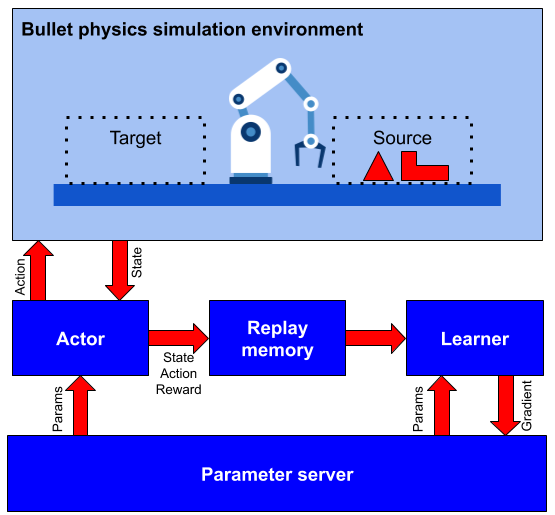
\includegraphics[scale=0.5]{simulation-arch}
	\caption{Standard simulation architecture}
	\label{fig:simulation-arch}
\end{figure}

To reduce training time, agent training via simulation is parallelized and distributed similar to GORILA architecture \cite{gorila}. In this project we use Ray RLLib \cite{rllib} which provides abstractions for distributed reinforcement learning.

\subsection{Simulation environment}
Simulation environment is developed using Bullet Physics simulator python module. Environment will be setup for a specific task like table clearing or stacking of objects. Environment will accept actions from specific task which must be in specific format according to action space of environment. When environment receives an action, it will apply the action to simulated environment using PyBullet APIs. After action is completed, the environment will record the state according to state space of environment and calculate the reward according to task setup of environment. Environment returns state and reward after action is applied.

\subsubsection{PyBullet Simulator}
PyBullet is a python module for Bullet Physics C SDK used for physics simulation in robotics, games, visual effects and machine learning, with a focus on sim-to-real transfer \cite{pybullet}. PyBullet can load visual, physical and other properties of a body from URDF, SDF and Mujoco formats. If required, 3D mesh of bodies can be loaded directly using PyBullet APIs. For simulating robots, PyBullet supports forward and inverse kinematics, collision detection, coordinate transformations, forward dynamics simulation, inverse dynamics computation, joint state position, velocity and force/torque control.

PyBullet supports rendering using CPU renderer and OpenGL renderer. Visualization can be optionally turned off in PyBullet. With visualization disabled, PyBullet uses CPU renderer for rendering images captured by camera API. This is especially useful in reinforcement learning where we want to collect data from simulated environment as fast as possible.

\subsection{Actor}
Actor is responsible for reading policy from the parameter server and execute actions is the simulation environment and save the action, returned state, returned reward in experience replay memory. When an actor is started, it will create a new simulation environment process. 
\begin{itemize}
	\item Start new simulation environment process
	\item Begin new episode
	\item Read policy ($\pi(a_t|s_t)$) and environment state ($s_t$). Evaluate and select action $a_t$ for state $s_t$ by evaluating policy $\pi(a_t|s_t)$. Execute the action $a_t$ on simulation environment environment and read the returned reward $r_t$ and new state of environment $s_{t+1}$. Save $[a_t, s_t, r_t, s_{t+1}]$ to replay buffer
	\item End episode when simulation environment terminates an episode
\end{itemize}

\subsection{Replay buffer}
Replay buffer stores the trajectory of episodes. Trajectory of an episode is a list of $[a_t, s_t, r_t, s_{t+1}]$. Since multiple actor process are supposed to add observations to replay buffer, replay buffer is usually a distributed database accessible by actor processes. We use redis in memory database is used as replay buffer database.

\subsection{Learner}
Learner reads the episode trajectories stored in replay buffer and optimize the policy stored in parameter server to maximize rewards. Learner process is specific to a reinforcement learning algorithm. Eg:- DDPG, PPO. Learner process uses deep learning frameworks like tensorflow or pytorch to model the policy, calculate the gradients for loss functions and do other computations.

\subsection{Parameter server}
Parameter server stores the policy. It is accessible by both actor and learner and also accepts gradient from learner and apply the gradient to update the policy represented by parameter server.

\section{Table Clearing Environment}
In table clearing environment, main components are a 6 axis ABB IRB 120 robot with MetalWork W155032001 parallel jaw gripper and a table with yellow and green tray. Object at random position and orientation is inserted into the source tray (yellow). The task is to move the object from source tray (yellow) to destination tray (green).

\begin{figure}[H]
	\centering
	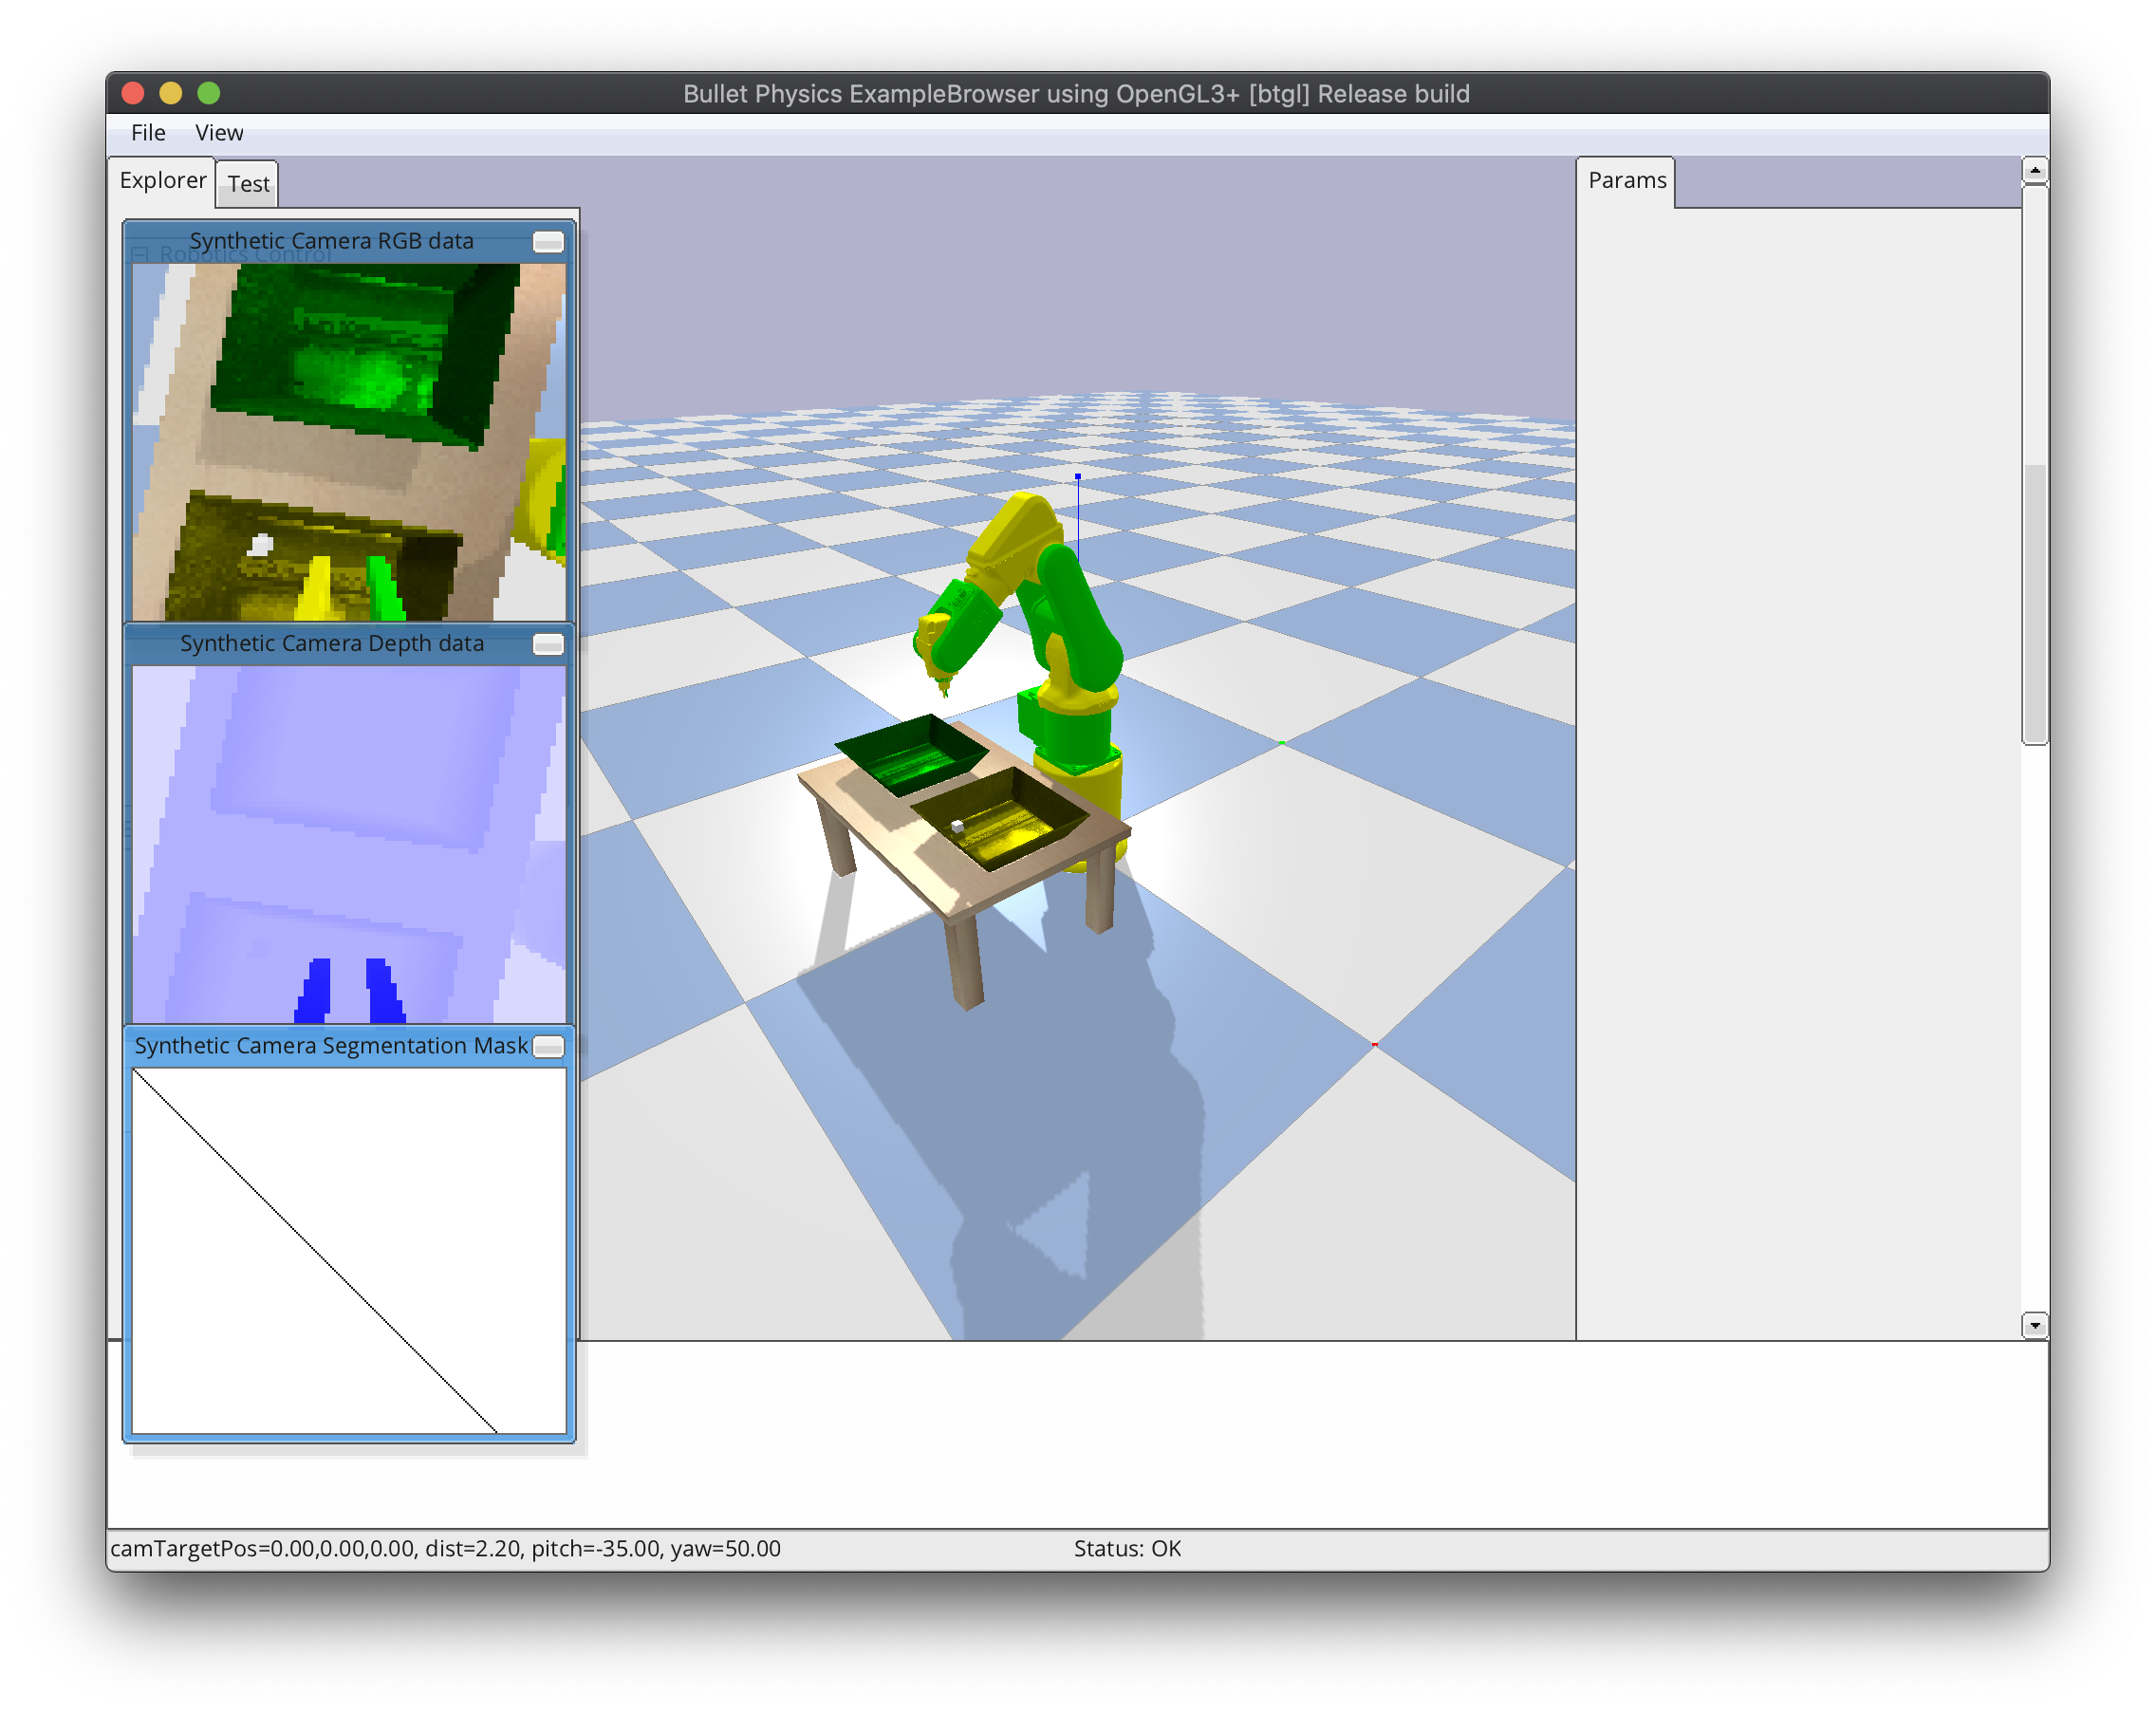
\includegraphics[scale=0.3]{table-clearing-env}
	\caption{Table clearing pybullet environment}
	\label{fig:table-clearing-env}
\end{figure}

\subsection{State space}
A RGB-D camera is mounted on the end effector of the gripper. The output of this camera is shown in lFigure \ref{fig:fig:table-clearing-env-camera}. The state space of the environment is a tensor of shape $84 \times 84 \times 4$. The first three channels are RGB pixel values and fourth channel is the depth value.

\begin{figure}[H]
	\centering
	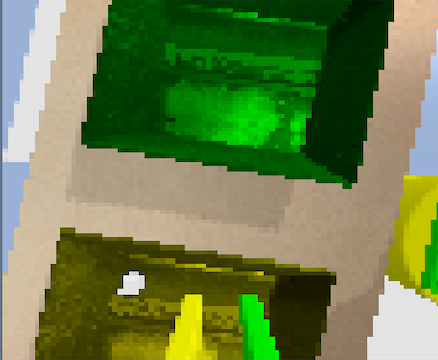
\includegraphics[scale=0.7]{table-clearing-rgb}
	
\includegraphics[scale=0.7]{table-clearing-depth}
	\caption{Gripper camera output; left: RGB, right: depth}
	\label{fig:fig:table-clearing-env-camera}
\end{figure}

\subsection{Action space}
\begin{figure}[H]
	\centering
	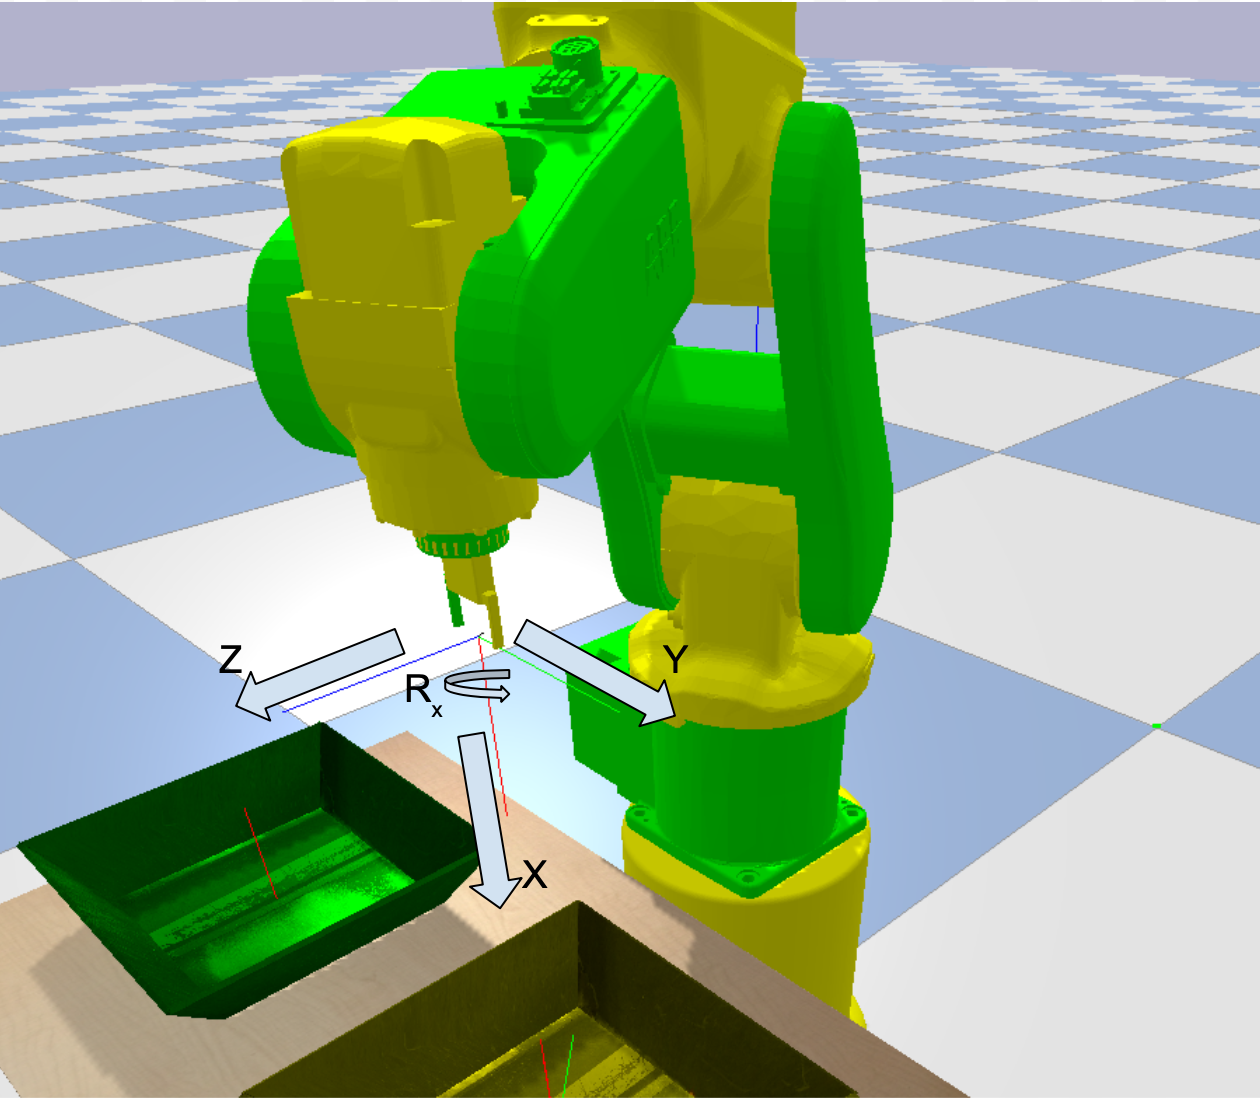
\includegraphics[scale=0.4]{table-clearing-env-action-space}
	\caption{Table clearing environment action coordinate system}
	\label{fig:table-clearing-env-action-space}
\end{figure}

The end effector position can be controlled by making $[\delta x, \delta y, \delta z]$ movements with respect to $X, Y \& Z$  axis of a coordinate system attached to gripper as shown in Figure \ref{fig:table-clearing-env-action-space}. The end effector can be rotated about approach vector by $\delta r_x$. The gripper fingers can be closed by setting binary variable $open$. The maximum/minimum values of a single action is shown in Table \ref{table:table-clearing-env-action-space}

\begin{table}[H]
	\centering
	\begin{tabular}{|c|c|}
		\hline 
		Action & Limit \\ 
		\hline 
		$\delta x, \delta y, \delta z$ & $[-1, 1]$ cm \\ 
		$\delta r_x$ & $[-10, 10] deg$ \\
		$open$ & {1, 0} \\
		\hline 
	\end{tabular}
	\caption{Table clearing environment action space}
	\label{table:table-clearing-env-action-space}
\end{table}

\subsection{Reward}
Let $s_t$ and $s_{t-1}$ be environment state at time $t$ and $t-1$ respectively. The total reward returned by the environment for action $a_t$ at time $t$ is the sum of following rewards

\begin{itemize}
	\item If object is not grasped and object has not moved far from initial position and gripper to object distance at time $t$ is less than $t-1$, reward is +1 else -1
	\item If object is grasped and gripper to destination tray distance at time $t$ is less than $t-1$, reward is +1 else -1
	\item For each action, reward of -1 is given to minimize time to complete task
	\item If body of robot including gripper touches any body other than target object, robot is assumed to be collided and a reward of -1000 is given
	\item If at time $t-1$, object is not grasped and at $t$, object is grasped, then a reward of +100 is given. Object is assumed to be grasped when target object is only in contact with gripper fingers and object is having a height of at least 5cm above source tray
	\item If at time $t-1$, object is grasped and at $t$, object is not grasped and target object is not at destination tray, object is assumed to be dropped and a reward of -200 is given
	\item If at time $t-1$, object is not at destination tray and at $t$, object is at destination tray, then object is assumed to be delivered and reward of +200 is given
\end{itemize}

\subsection{Episode termination}
A simulation episode is terminated at following conditions
\begin{itemize}
	\item Robot or gripper body is in contact with any body other than target object (collision)
	\item Target object reached destination tray (delivered)
	\item Duration of episode is greater than 3 minutes
	\item Number of actions taken in episode is greater than 3000
\end{itemize}
